\textbf{Целью третьей лабораторной работы} является отработка навыков использования программы Microsoft Project для оптимизации временных и финансовых показателей проекта.

\section*{Содержание проекта}

Команда разработчиков из 16 человек занимается созданием карты города на основе собственного модуля отображения. Проект должен быть завершен в течение шести месяцев. Бюджет проекта: 50 000 рублей.

\section*{Сведения о ресурсах проекта}

На рисунке \ref{img:task1-start-overload} представлены существующие в проекте перегрузки.

\begin{figure}[H]
	\begin{center}
		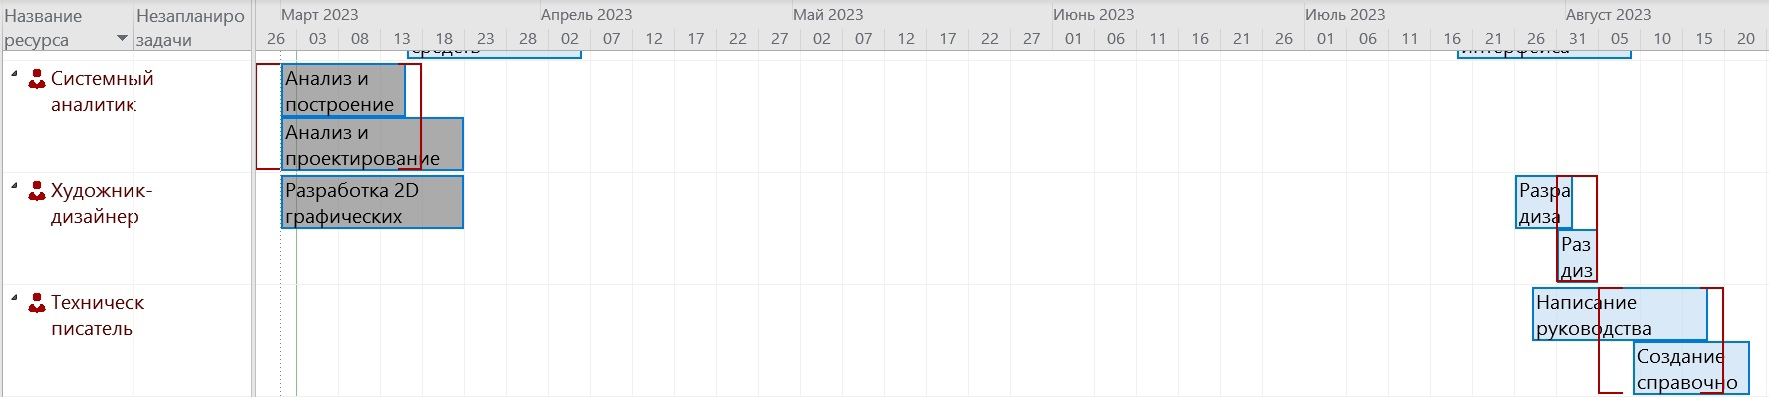
\includegraphics[scale=0.26]{inc/img/task1-start-overload.jpg}
	\end{center}
	\captionsetup{justification=centering}
	\caption{Существующие в проекте перегрузки}
	\label{img:task1-start-overload}
\end{figure}

Перегрузки для ресурса <<Системный аналитик>> связаны с тем, что данный ресурс задействован при выполнении задач <<Анализ и построение структуры базы объектов>> и <<Анализ и проектирование ядра>>, сроки реализаций которых накладываются.

Перегрузки для ресурса <<Художник-дизайнер>> связаны с тем, что данный ресурс задействован при выполнении задач <<Разработка дизайна руководства>> и <<Разработка дизайна сайта>>, сроки реализаций которых накладываются.

Перегрузки для ресурса <<Технический писатель>> связаны с тем, что данный ресурс задействован при выполнении задач <<Написание руководства пользователя>> и <<Создание справочной системы>>, сроки реализаций которых накладываются.

Устранить перегрузки можно следующими способами:

\begin{itemize}
	\item изменить календарь работы ресурса;
	\item назначить ресурс на неполный рабочий день;
	\item изменить профиль назначения ресурса;
	\item изменить ставку оплаты ресурса;
	\item добавить ресурсу время задержки;
	\item разбить задачу на этапы и перекрыть по времени их выполнение;
	\item применить автоматическое выравнивание.
\end{itemize}

\section*{Задание 1}

Так как в проекте перегружено несколько ресурсов, для устранения перегрузок использовалось автоматическое выравнивание. Параметры выравнивания приведены на рисунке \ref{img:task1-alignment}.

\begin{figure}[H]
	\begin{center}
		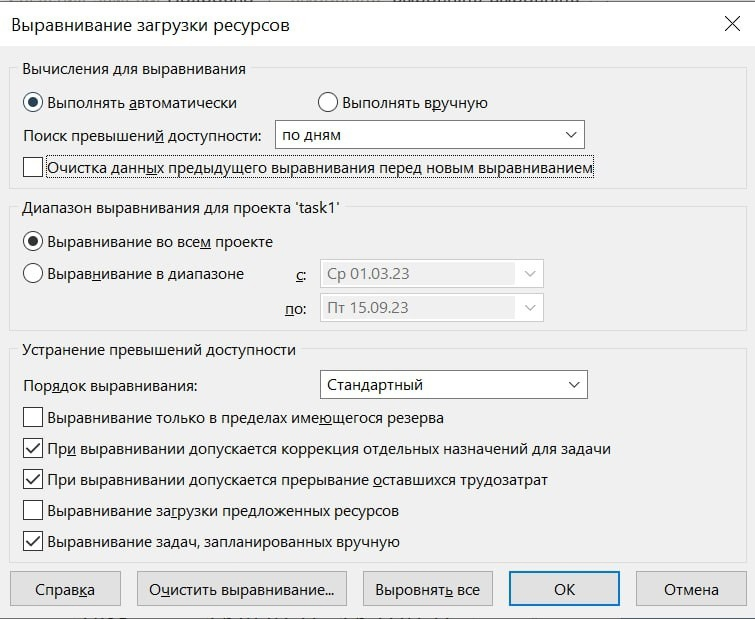
\includegraphics[scale=0.45]{inc/img/task1-alignment.jpg}
	\end{center}
	\captionsetup{justification=centering}
	\caption{Параметры выравнивания}
	\label{img:task1-alignment}
\end{figure}

После применения автоматического выравнивания бюджет проекта не изменился, а дата завершения проекта сдвинулась с 15.09.2023 на 19.09.2023, что показано на рисунке \ref{img:task1-state}.

\begin{figure}[H]
	\begin{center}
		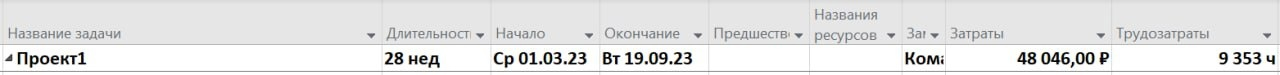
\includegraphics[scale=0.3]{inc/img/task1-state.jpg}
	\end{center}
	\captionsetup{justification=centering}
	\caption{Сведения проекта после выравнивания}
	\label{img:task1-state}
\end{figure}

Полученная после выравнивания диаграмма Ганта представлена на рисунке \ref{img:task1-diagram}.

\begin{figure}[H]
	\begin{center}
		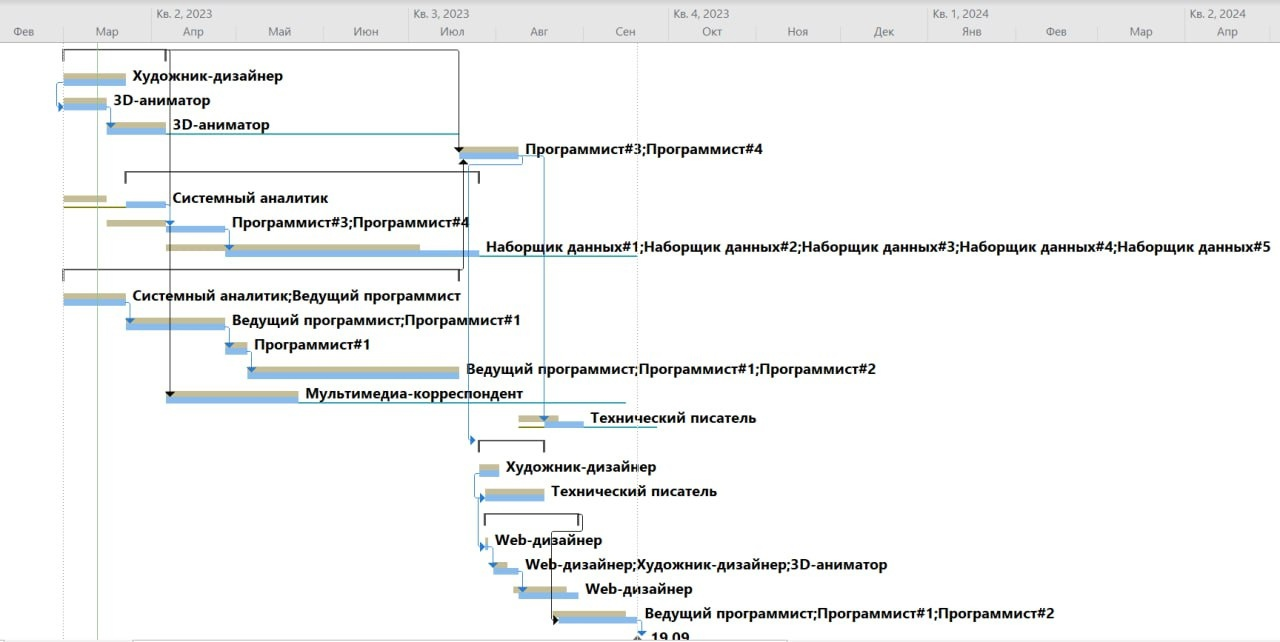
\includegraphics[scale=0.3]{inc/img/task1-diagram.jpg}
	\end{center}
	\captionsetup{justification=centering}
	\caption{Полученная после выравнивания диаграмма Ганта}
	\label{img:task1-diagram}
\end{figure}

На визуальном оптимизаторе ресурсов видно, что ресурсы не перегружены (рисунок \ref{img:task1-recources}).

\begin{figure}[H]
	\begin{center}
		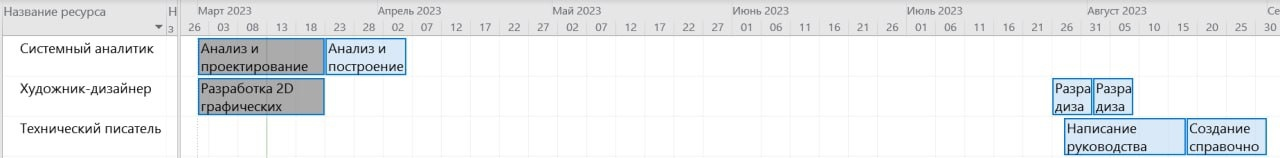
\includegraphics[scale=0.3]{inc/img/task1-resources.jpg}
	\end{center}
	\captionsetup{justification=centering}
	\caption{Визуальный оптимизатор ресурсов после выравнивания}
	\label{img:task1-recources}
\end{figure}
 
Перегрузки для ресурса <<Системный аналитик>> были решены за счет переноса начала задачи <<Анализ и построение структуры базы объектов>> (рисунки \ref{img:task1-analysis-before} и \ref{img:task1-analysis-after}). Так как эта задача не входит в критический путь, этот сдвиг не повлиял на длительность проекта, но позволил решить перегрузку.

\begin{figure}[H]
	\begin{center}
		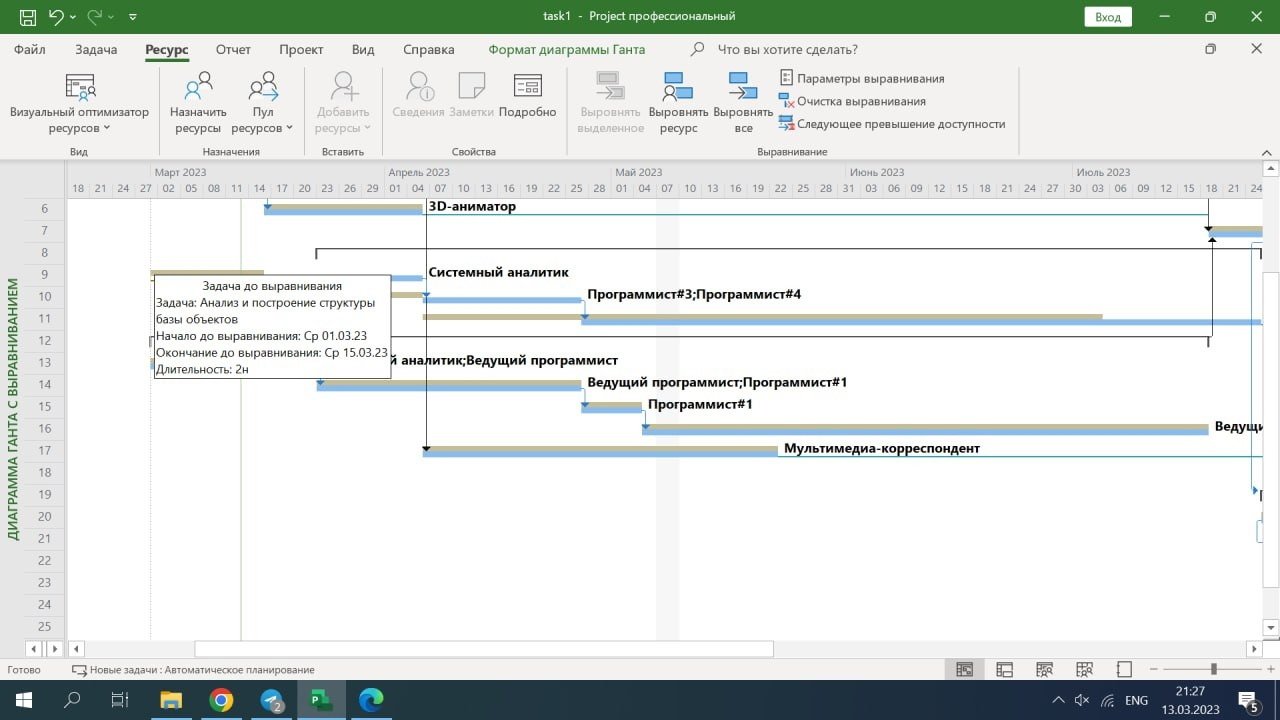
\includegraphics[scale=0.3]{inc/img/task1-analysis-before.jpg}
	\end{center}
	\captionsetup{justification=centering}
	\caption{Задача <<Анализ и построение структуры базы объектов>> до выравнивания}
	\label{img:task1-analysis-before}
\end{figure}

\begin{figure}[H]
	\begin{center}
		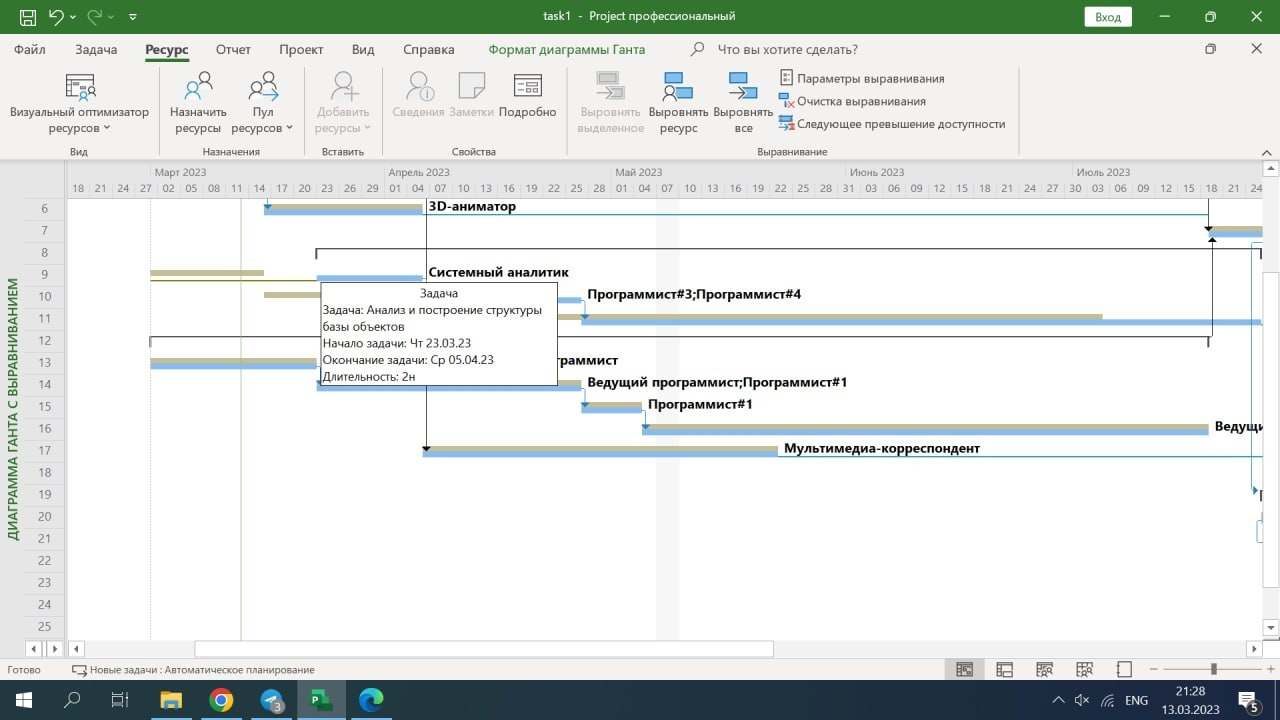
\includegraphics[scale=0.3]{inc/img/task1-analysis-after.jpg}
	\end{center}
	\captionsetup{justification=centering}
	\caption{Задача <<Анализ и построение структуры базы объектов>> после выравнивания}
	\label{img:task1-analysis-after}
\end{figure}

Перегрузки для ресурса <<Художник-дизайнер>> были решены за счет задержки выполнения задачи <<Разработка дизайна сайта>> (рисунки \ref{img:task1-designer-before} и \ref{img:task1-designer-after}).

\begin{figure}[H]
	\begin{center}
		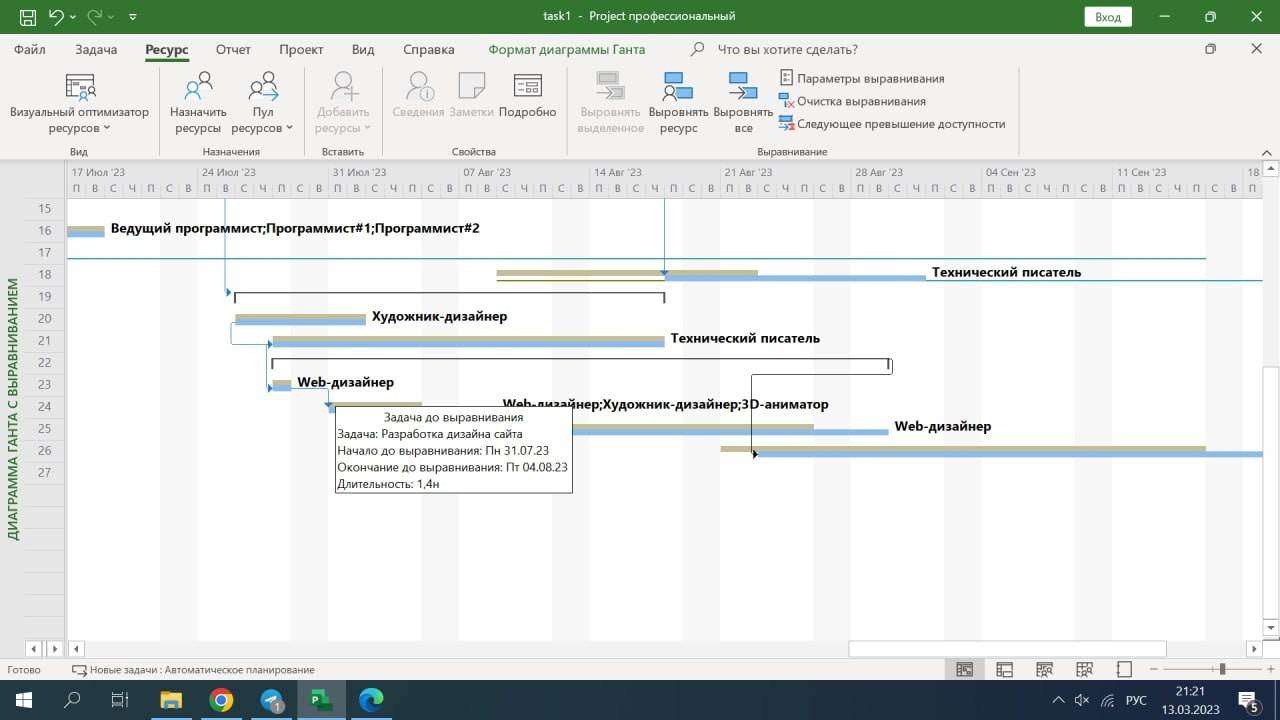
\includegraphics[scale=0.3]{inc/img/task1-designer-before.jpg}
	\end{center}
	\captionsetup{justification=centering}
	\caption{Задача <<Разработка дизайна сайта>> до выравнивания}
	\label{img:task1-designer-before}
\end{figure}

\begin{figure}[H]
	\begin{center}
		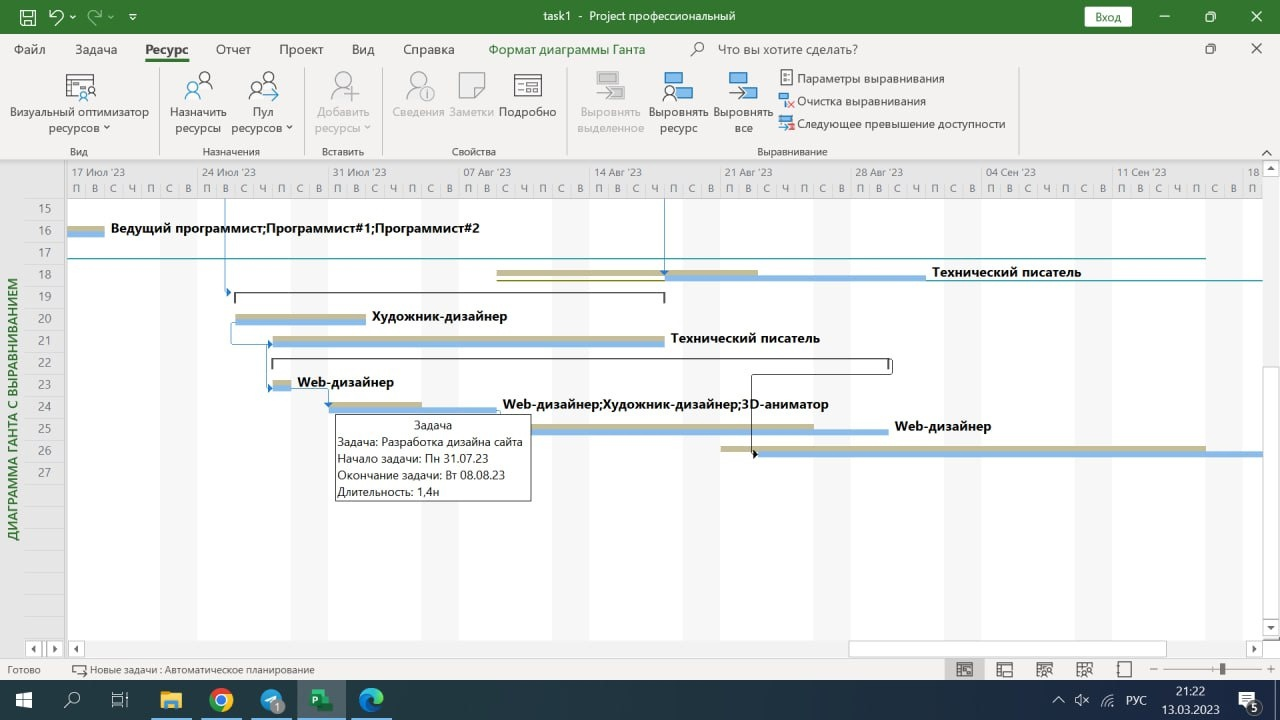
\includegraphics[scale=0.3]{inc/img/task1-designer-after.jpg}
	\end{center}
	\captionsetup{justification=centering}
	\caption{Задача <<Разработка дизайна сайта>> после выравнивания}
	\label{img:task1-designer-after}
\end{figure}

Перегрузки для ресурса <<Технический писатель>> были решены за счет переноса начала задачи <<Создание справочной системы>> (рисунки \ref{img:task1-writer-before} и \ref{img:task1-writer-after}). Данная задача входит в критический путь, поэтому сдвиг влияет на длительность проекта.

\begin{figure}[H]
	\begin{center}
		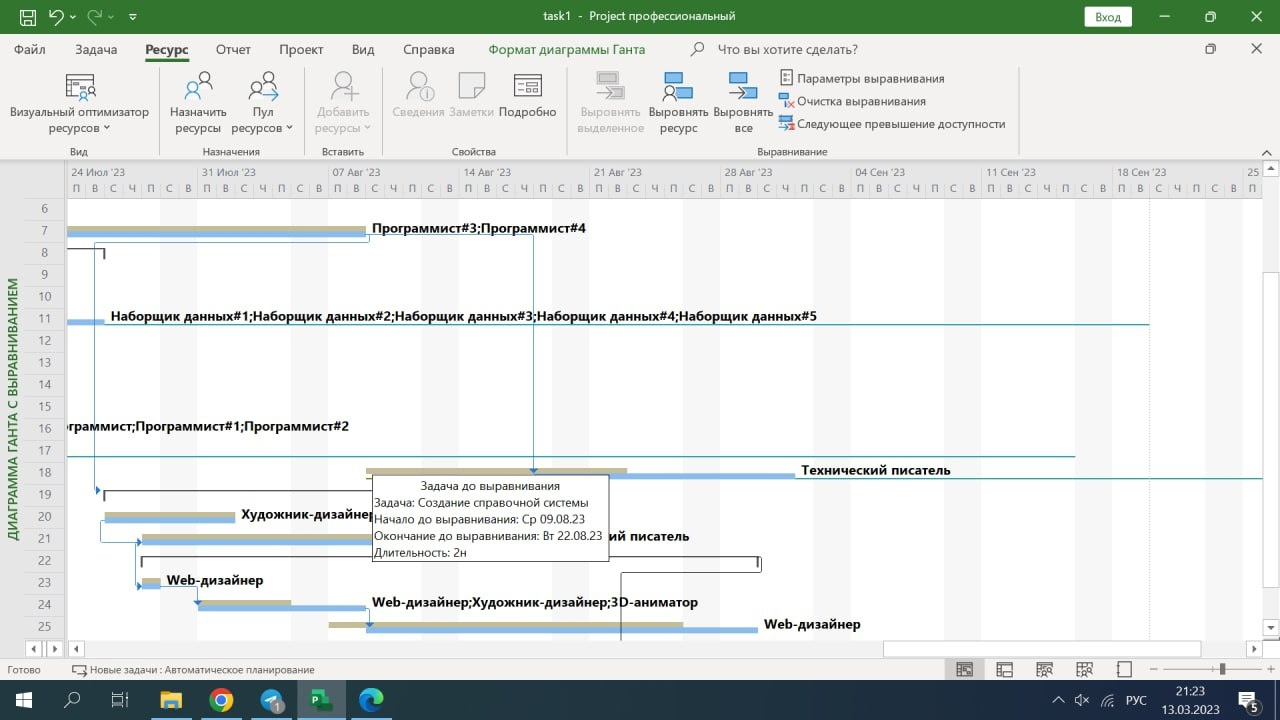
\includegraphics[scale=0.3]{inc/img/task1-writer-before.jpg}
	\end{center}
	\captionsetup{justification=centering}
	\caption{Задача <<Создание справочной системы>> до выравнивания}
	\label{img:task1-writer-before}
\end{figure}

\begin{figure}[H]
	\begin{center}
		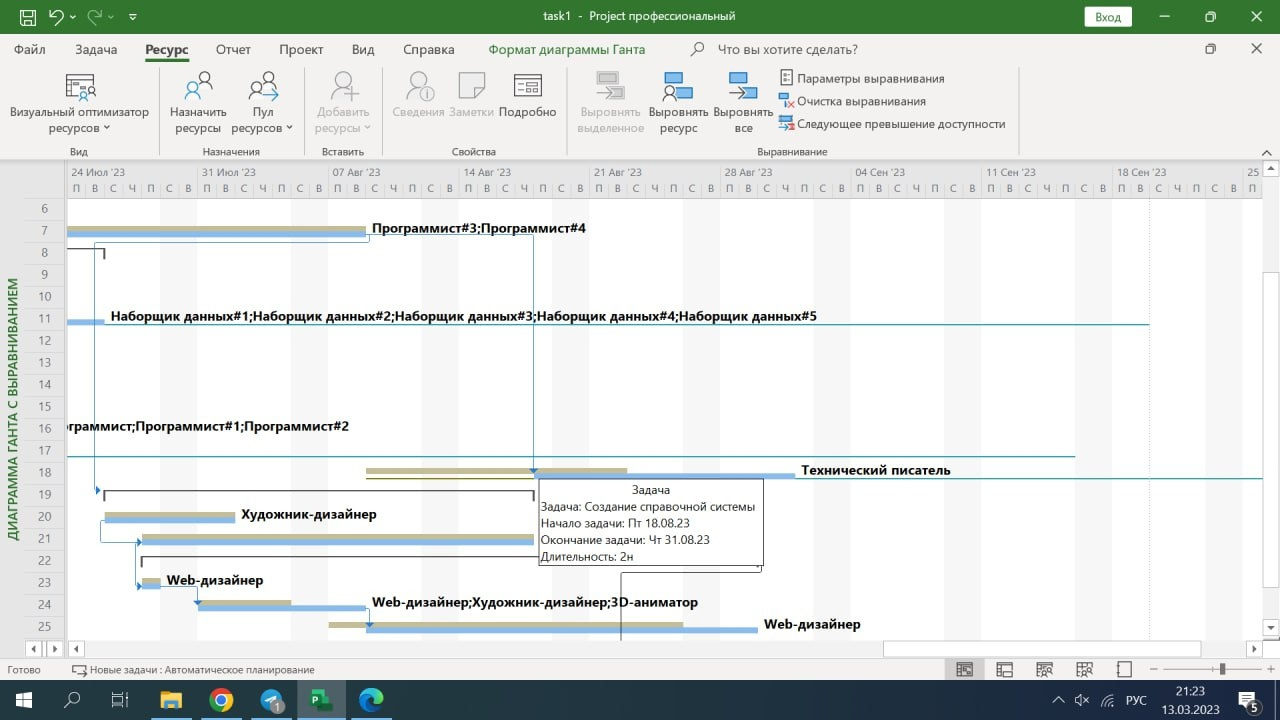
\includegraphics[scale=0.3]{inc/img/task1-writer-after.jpg}
	\end{center}
	\captionsetup{justification=centering}
	\caption{Задача <<Создание справочной системы>> после выравнивания}
	\label{img:task1-writer-after}
\end{figure}

\section*{Задание 2}

Была добавлена повторяющаяся задача <<Совещание>>  с параметрами, приведенными на рисунке \ref{img:task2-meeting}. Данная задача в списке задач показана на рисунке \ref{img:task2-list-meeting}.

\begin{figure}[H]
	\begin{center}
		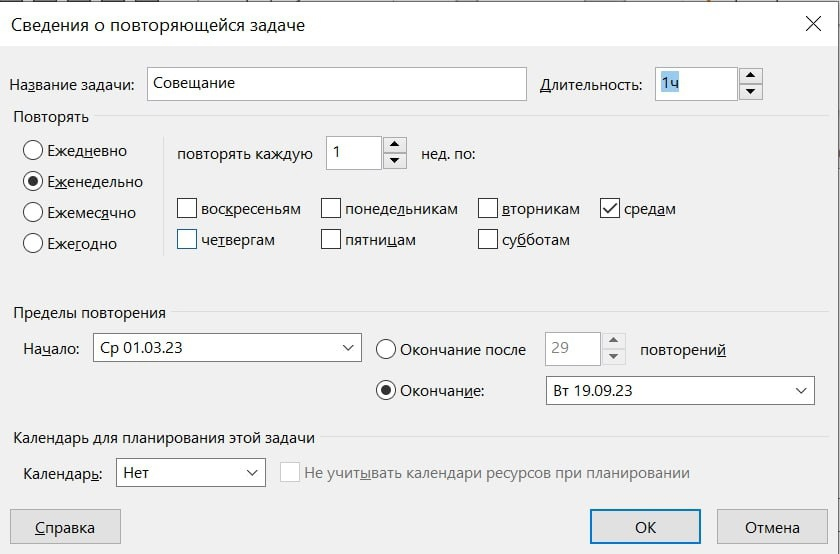
\includegraphics[scale=0.3]{inc/img/task2-meeting.jpg}
	\end{center}
	\captionsetup{justification=centering}
	\caption{Создание повторяющейся задачи <<Совещание>>}
	\label{img:task2-meeting}
\end{figure}

\begin{figure}[H]
	\begin{center}
		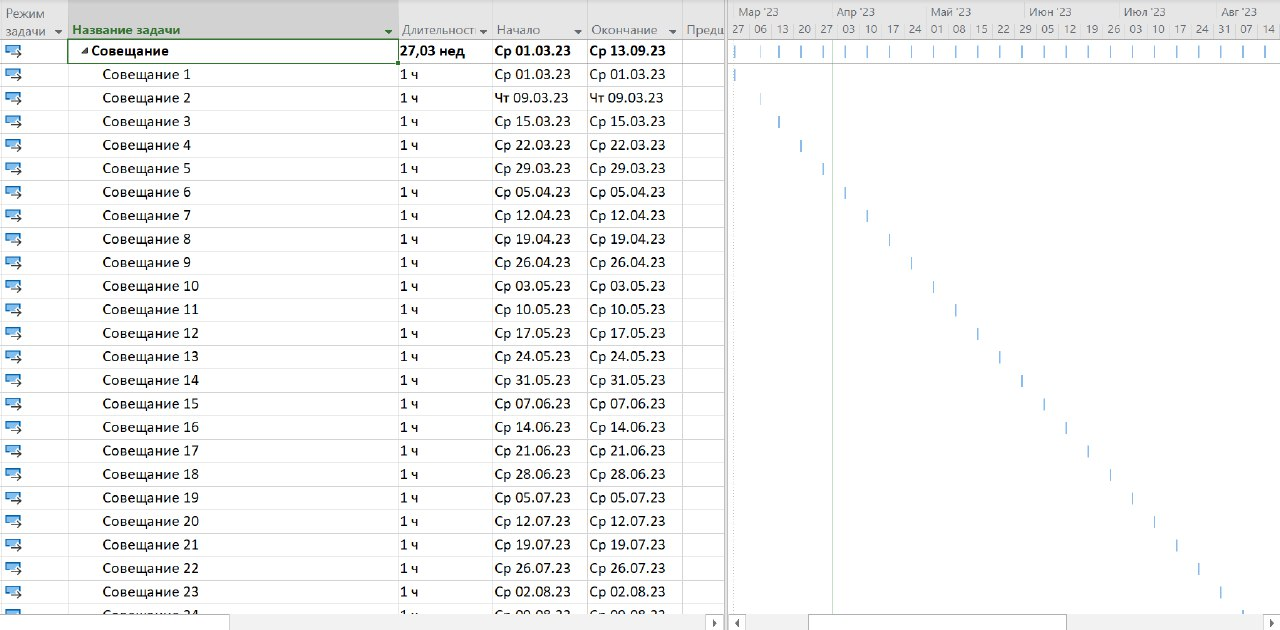
\includegraphics[scale=0.4]{inc/img/task2-list-meeting.jpg}
	\end{center}
	\captionsetup{justification=centering}
	\caption{Повторяющаяся задача <<Совещание>> в списке задач}
	\label{img:task2-list-meeting}
\end{figure}

Повторяющейся задаче были назначены ресурсы, как показано на рисунке \ref{img:task2-resources}.

\begin{figure}[H]
	\begin{center}
		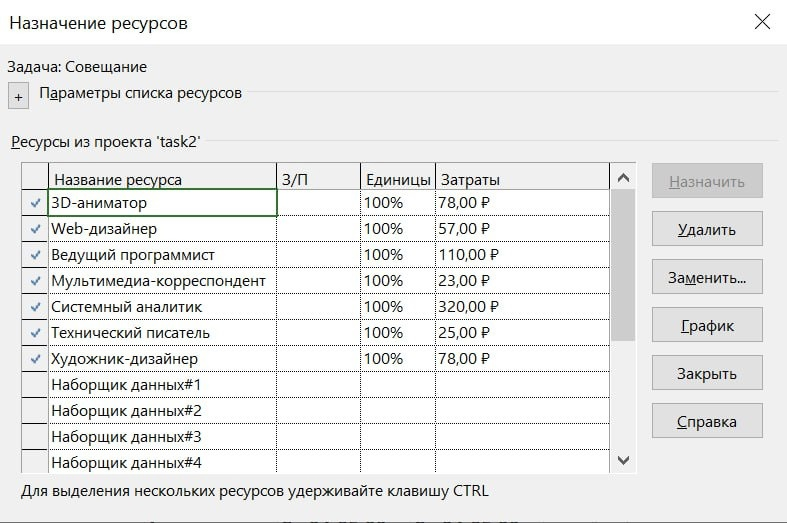
\includegraphics[scale=0.25]{inc/img/task2-resources.jpg}
	\end{center}
	\captionsetup{justification=centering}
	\caption{Назначение ресурсов повторяющейся задаче <<Совещание>>}
	\label{img:task2-resources}
\end{figure}

Затраты и трудозатраты на повторяющуюся задачу <<Совещание>> составили 20 039 рублей и 203 часа, как представлено на рисунке \ref{img:task2-meeting-costs}.

\begin{figure}[H]
	\begin{center}
		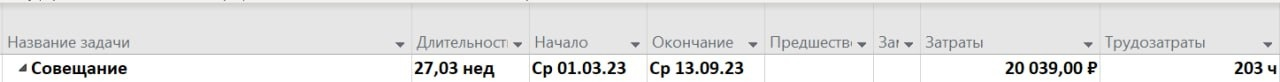
\includegraphics[scale=0.3]{inc/img/task2-meeting-costs.jpg}
	\end{center}
	\captionsetup{justification=centering}
	\caption{Затраты и трудозатраты на повторяющуюся задачу <<Совещание>>}
	\label{img:task2-meeting-costs}
\end{figure}

Затраты и трудозатраты проекта после добавления повторяющейся задачи <<Совещание>> составили 68 085 рублей и 9 556 часов, что приведено на рисунке \ref{img:task2-meeting-budget}. Затраты на проект превышают заявленный бюджет, равный 50 000 рублей.

\begin{figure}[H]
	\begin{center}
		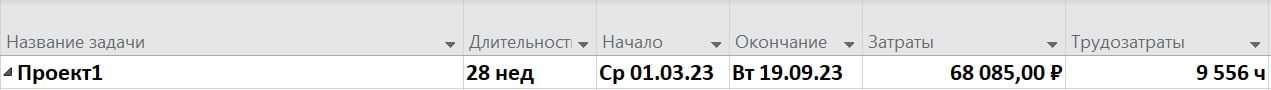
\includegraphics[scale=0.3]{inc/img/task2-meeting-budget.jpg}
	\end{center}
	\captionsetup{justification=centering}
	\caption{Затраты и трудозатраты проекта после добавления повторяющейся задачи}
	\label{img:task2-meeting-budget}
\end{figure}

В связи с тем, что совещания происходили во время работы сотрудников возникли перегрузки, показанные на рисунке \ref{img:task2-meeting-overload}. 

\begin{figure}[H]
	\begin{center}
		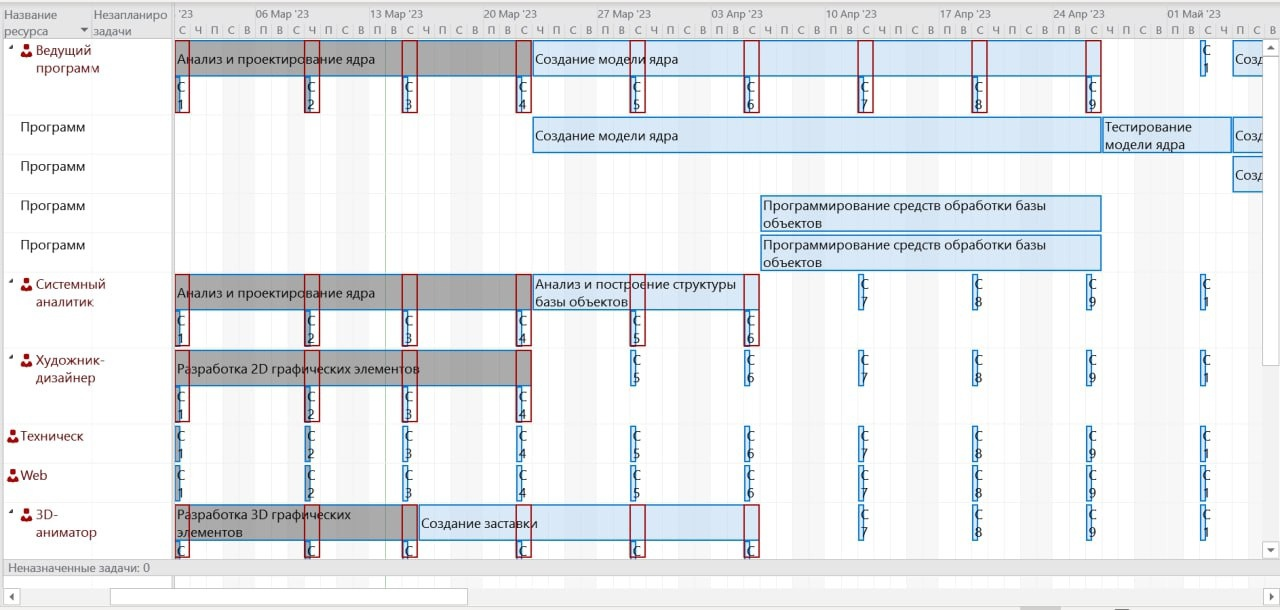
\includegraphics[scale=0.3]{inc/img/task2-meeting-overload.jpg}
	\end{center}
	\captionsetup{justification=centering}
	\caption{Возникшие перегрузки}
	\label{img:task2-meeting-overload}
\end{figure}

Так как в проекте перегружено несколько ресурсов, для устранения перегрузок использовалось автоматическое выравнивание. Статистика проекта после выравнивания представлена на рисунке \ref{img:task2-alignment}. Были добавлены перерывы в выполнении задач для совещаний, из-за этого срок завершения проекта сдвинулся на 22.09.2023.

\begin{figure}[H]
	\begin{center}
		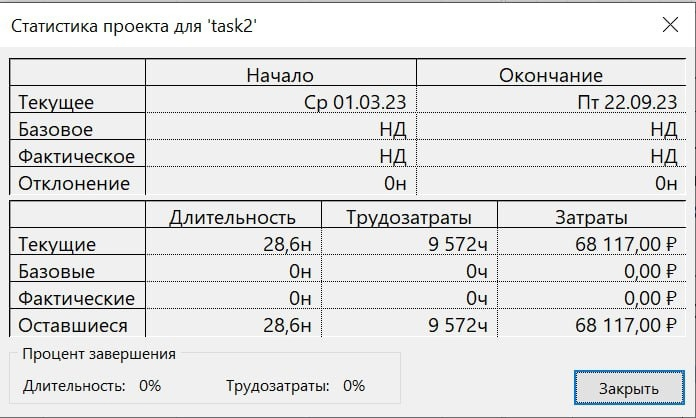
\includegraphics[scale=0.3]{inc/img/task2-alignment.jpg}
	\end{center}
	\captionsetup{justification=centering}
	\caption{Статистика проекта после выравнивания}
	\label{img:task2-alignment}
\end{figure}

Так как значения бюджета превышено, была проведена оптимизация параметров проекта. Во время совещаний сотрудники не использовали свои рабочие места, поэтому были сокращены затраты на использование этих сотрудников. Для этого был настроен другой план оплаты, что приведено на рисунках \ref{img:task2-b} и \ref{img:task2-b2}.

\begin{figure}[H]
	\begin{center}
		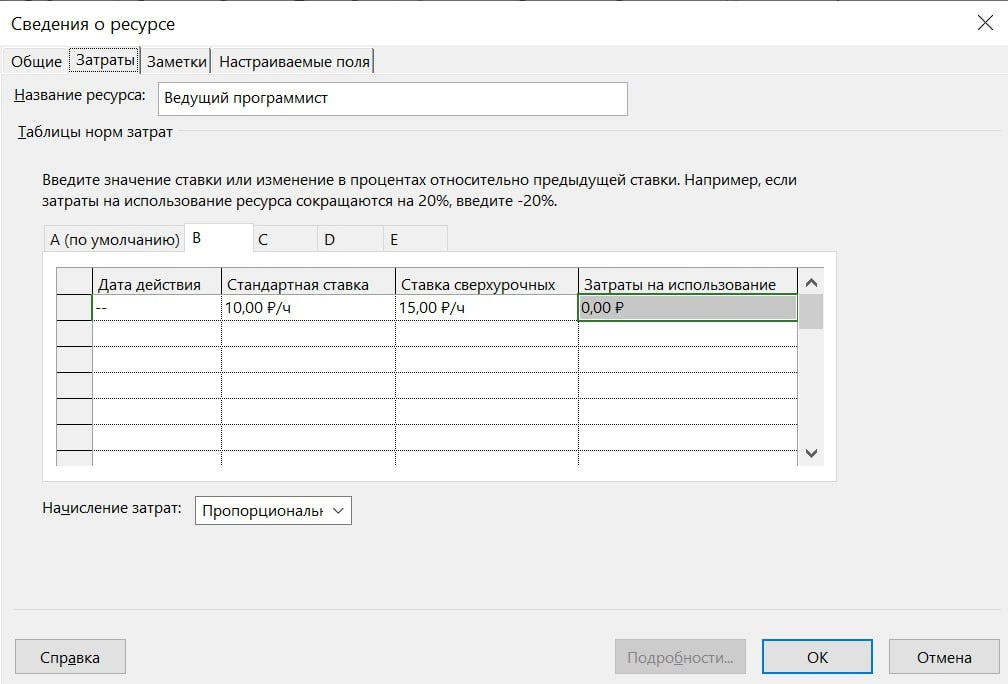
\includegraphics[scale=0.3]{inc/img/task2-b.jpg}
	\end{center}
	\captionsetup{justification=centering}
	\caption{Настройка другого плана оплаты}
	\label{img:task2-b}
\end{figure}

\begin{figure}[H]
	\begin{center}
		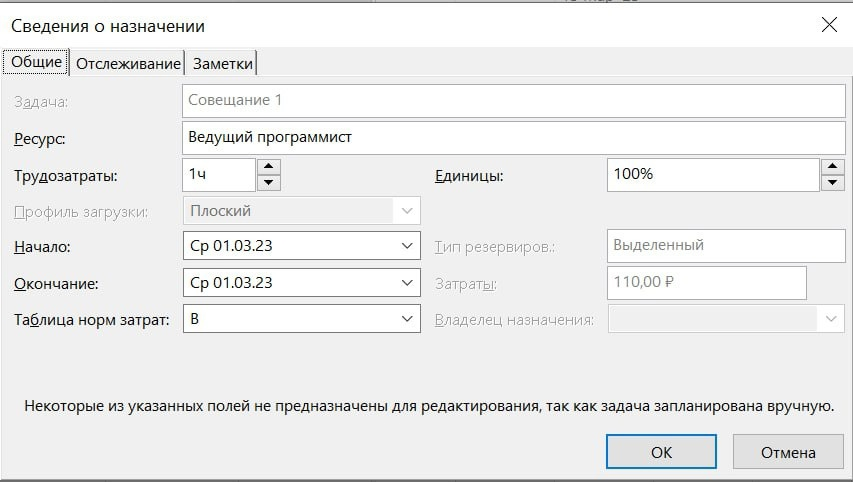
\includegraphics[scale=0.3]{inc/img/task2-b2.jpg}
	\end{center}
	\captionsetup{justification=centering}
	\caption{Настройка другого плана оплаты}
	\label{img:task2-b2}
\end{figure}

После этого затраты на совещания снизились до 1 769 рублей, как показано на рисунке \ref{img:task2-low}.

\begin{figure}[H]
	\begin{center}
		
\includegraphics[scale=0.3]{inc/img/task2-low.jpg}
	\end{center}
	\captionsetup{justification=centering}
	\caption{Обновленные затраты на совещания}
	\label{img:task2-low}
\end{figure}

Бюджет проекта уменьшился до 49 847 р, что укладывается в заявленные 50 000 р (рисунок \ref{img:task2-low-budget}).

\begin{figure}[H]
	\begin{center}
		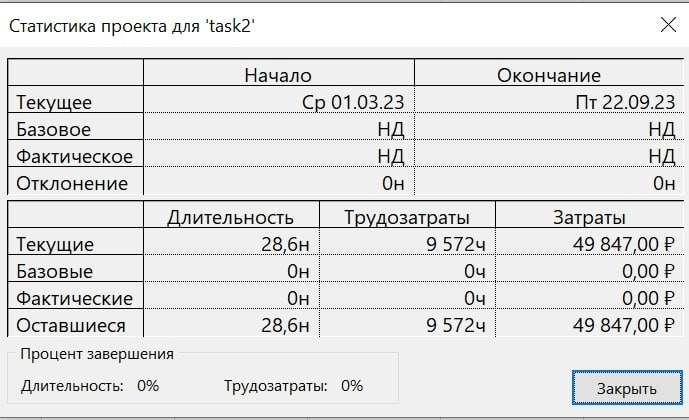
\includegraphics[scale=0.3]{inc/img/task2-low-budget.jpg}
	\end{center}
	\captionsetup{justification=centering}
	\caption{Состояние проекта после оптимизации затрат}
	\label{img:task2-low-budget}
\end{figure}

\section*{Задание 3}

На критическом пути, представленном на рисунке \ref{img:task3-critical}, одними из самых длинных являются задачи, связанные с программированием. При уменьшение их длительности уменьшилась бы и длительность всего проекта.

\begin{figure}[H]
	\begin{center}
		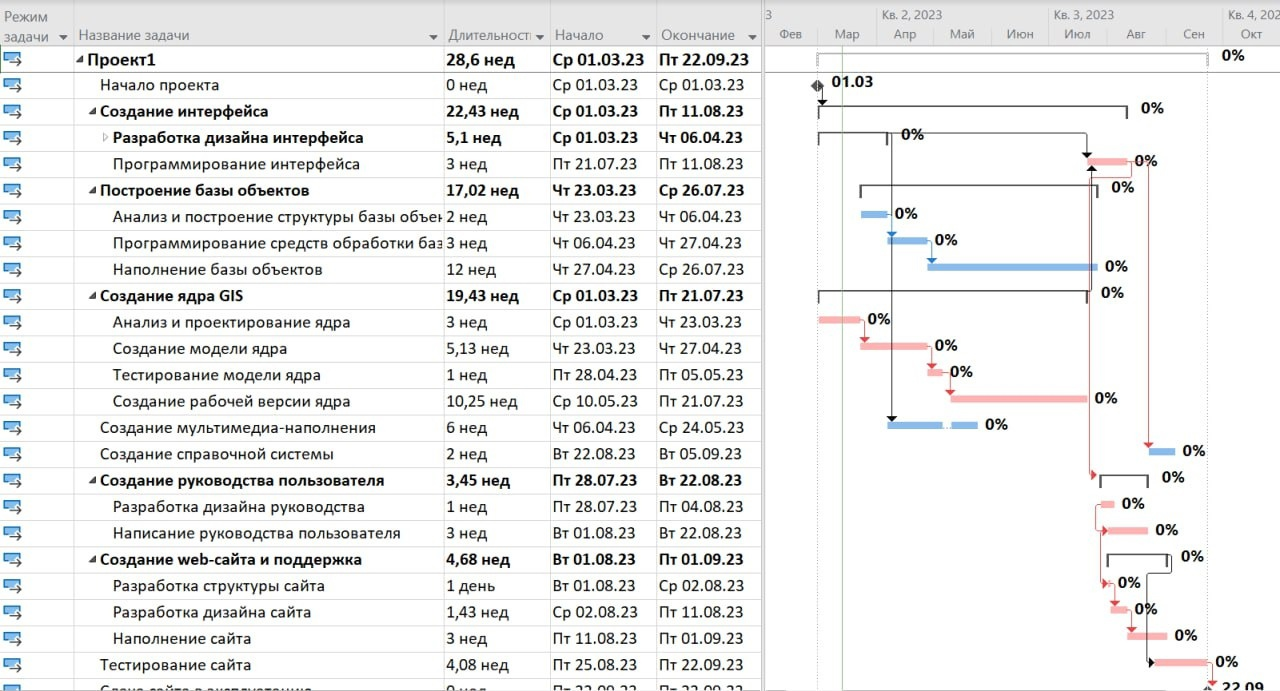
\includegraphics[scale=0.3]{inc/img/task3-critical.jpg}
	\end{center}
	\captionsetup{justification=centering}
	\caption{Критический путь проекта}
	\label{img:task3-critical}
\end{figure}

Как показано на рисунке \ref{img:task3-programmers-before}, на задачах, связанных с программированием, зачастую работают не все программисты. Можно назначить дополнительных программистов на задачи и уменьшить тем самым длительность задач.

\begin{figure}[H]
	\begin{center}
		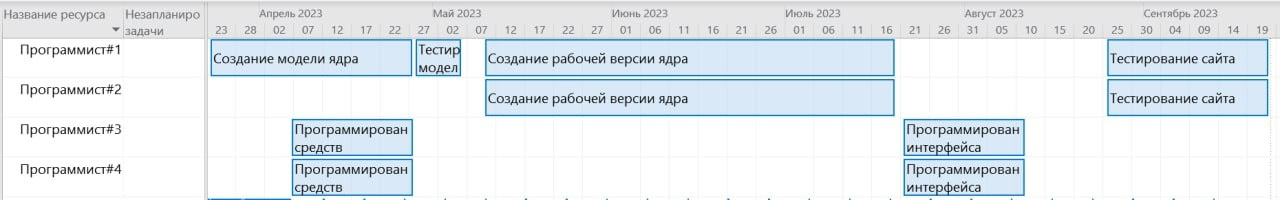
\includegraphics[scale=0.3]{inc/img/task3-programmers-before.jpg}
	\end{center}
	\captionsetup{justification=centering}
	\caption{Занятость программистов}
	\label{img:task3-programmers-before}
\end{figure}

Пример назначения программистов на задачи критического пути, в которых задействованы не все программисты, приведено на рисунке \ref{img:task3-resources}.

\begin{figure}[H]
	\begin{center}
		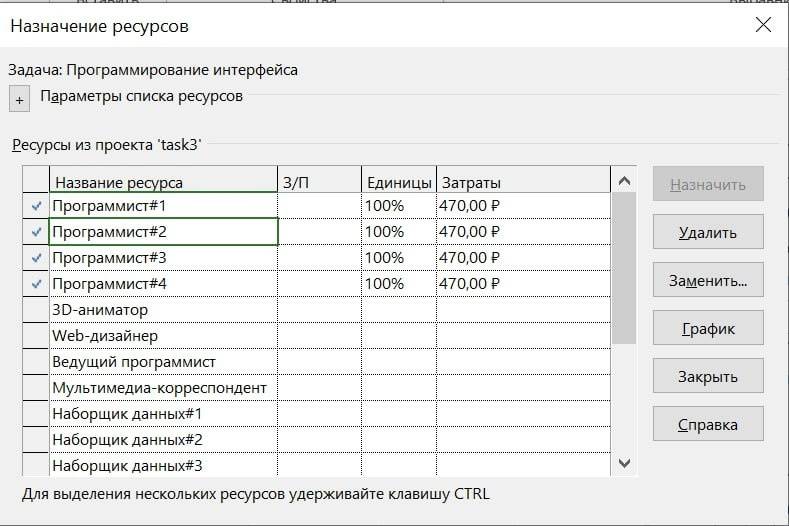
\includegraphics[scale=0.25]{inc/img/task3-resources.jpg}
	\end{center}
	\captionsetup{justification=centering}
	\caption{Назначение всех программистов на задачу <<Программирование интерфейса>>}
	\label{img:task3-resources}
\end{figure}

Полученная занятость работников представлена на рисунке \ref{img:task3-programmers-after}. Теперь программисты заняты более равномерно и большую часть времени работают все четверо.

\begin{figure}[H]
	\begin{center}
		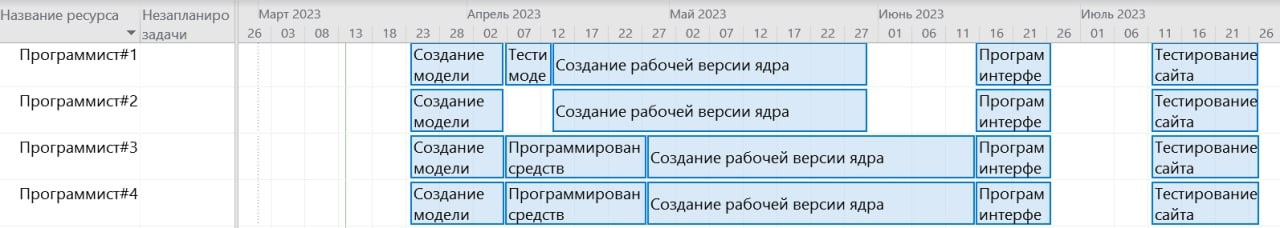
\includegraphics[scale=0.3]{inc/img/task3-programmers-after.jpg}
	\end{center}
	\captionsetup{justification=centering}
	\caption{Занятость программистов}
	\label{img:task3-programmers-after}
\end{figure}

После оптимизаций были удалены совещания, которые происходят после завершения последней задачи, оставшиеся совещания --- на рисунке \ref{img:task3-delete}.

\begin{figure}[H]
	\begin{center}
		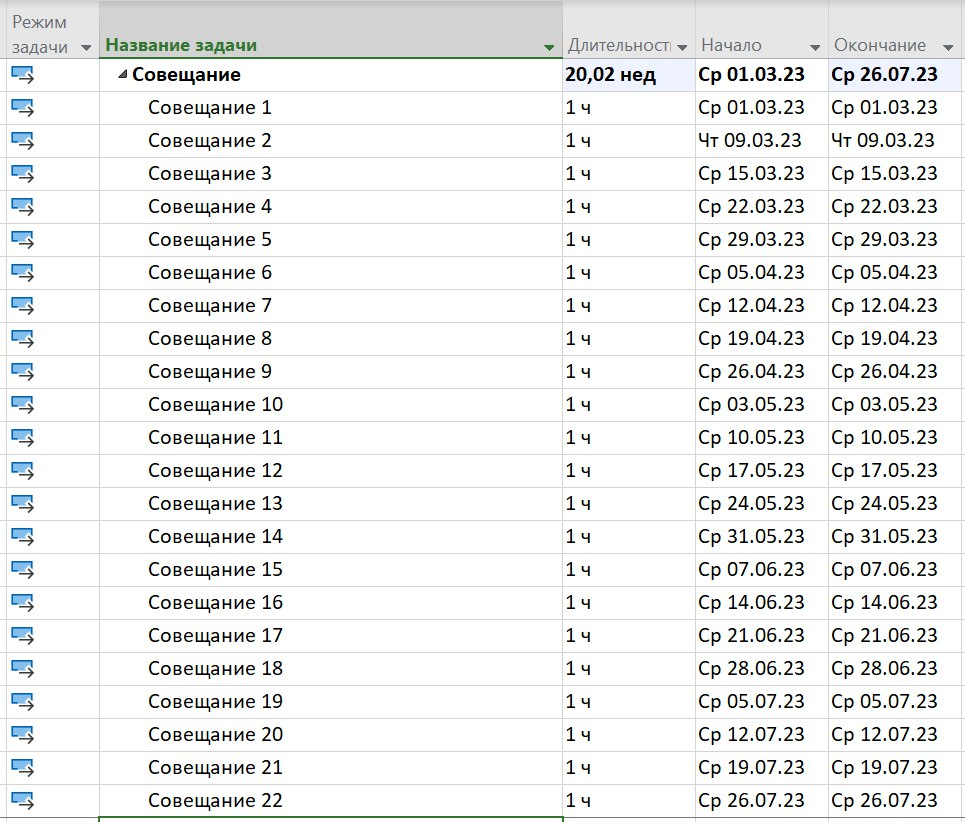
\includegraphics[scale=0.3]{inc/img/task3-delete.jpg}
	\end{center}
	\captionsetup{justification=centering}
	\caption{Оставшиеся в проекте совещания}
	\label{img:task3-delete}
\end{figure}

После добавления дополнительных программистов к задачам, дата сдвинулась на 27.07.2023, а затраты стали равными 48 824.57 рублей. Теперь проект удовлетворяет требованиям по срокам реализации и бюджету, что показано на рисунке \ref{img:task3-final}.

\begin{figure}[H]
	\begin{center}
		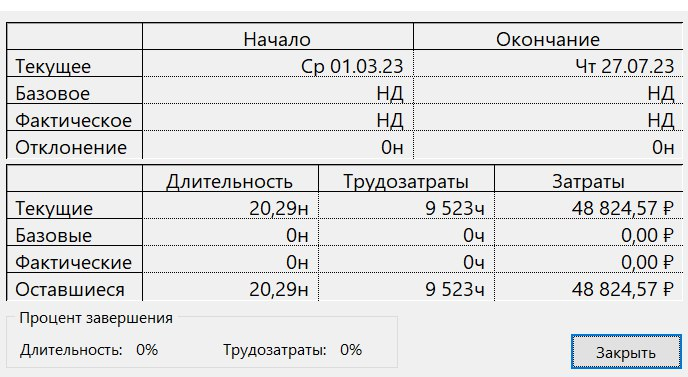
\includegraphics[scale=0.3]{inc/img/task3-final.jpg}
	\end{center}
	\captionsetup{justification=centering}
	\caption{Статистика проекта}
	\label{img:task3-final}
\end{figure}

Была проведена структуризация затрат по группам ресурсов, как приведено на рисунке \ref{img:task3-new-costs}. Графическое представление информации о затратах по структурным группам ресурсов показано на рисунке \ref{img:task3-graph-costs}.

\begin{figure}[H]
	\begin{center}
		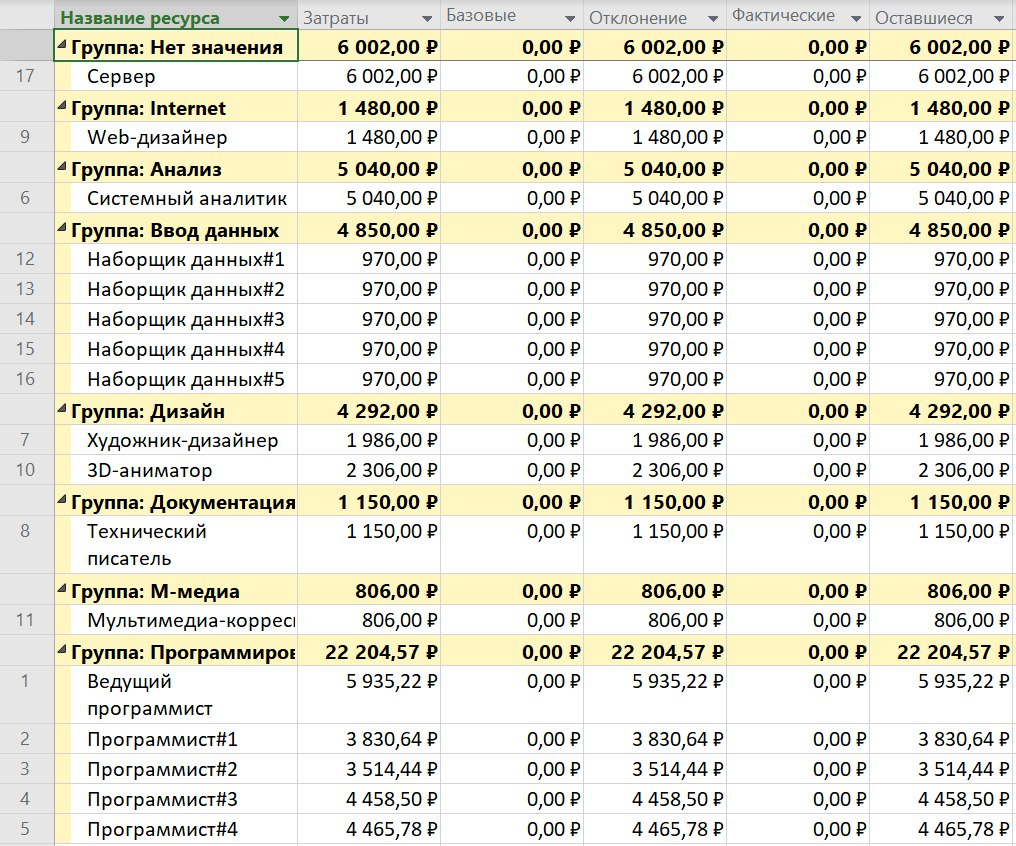
\includegraphics[scale=0.3]{inc/img/task3-new-costs.jpg}
	\end{center}
	\captionsetup{justification=centering}
	\caption{Структуризация затрат по группам ресурсов}
	\label{img:task3-new-costs}
\end{figure}

\begin{figure}[H]
	\begin{center}
		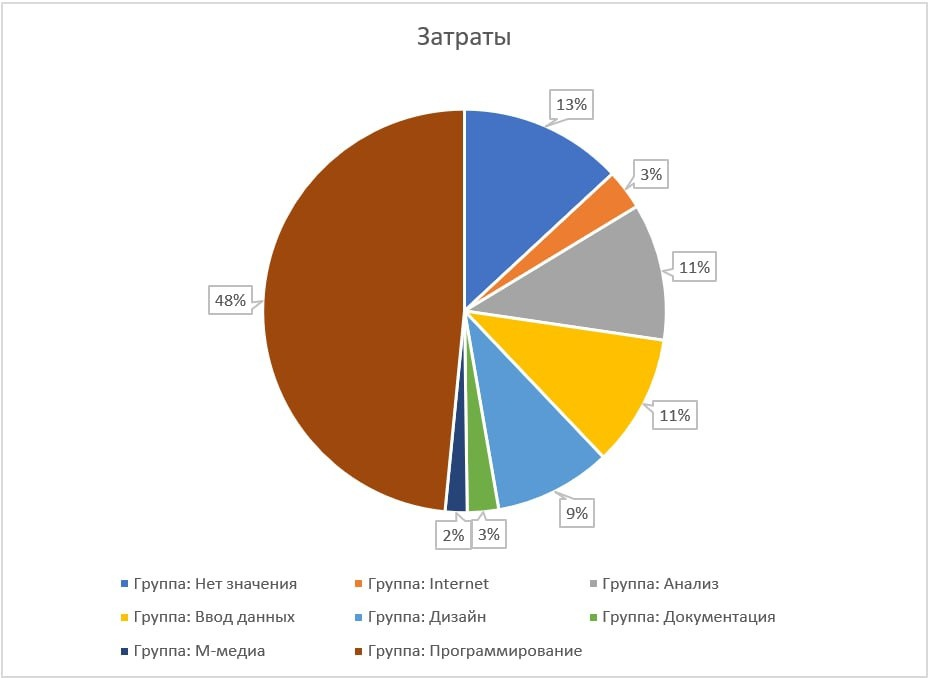
\includegraphics[scale=0.4]{inc/img/task3-graph-costs.jpg}
	\end{center}
	\captionsetup{justification=centering}
	\caption{Информации о затратах по структурным группам ресурсов}
	\label{img:task3-graph-costs}
\end{figure}

\begin{figure}[H]
	\begin{center}
		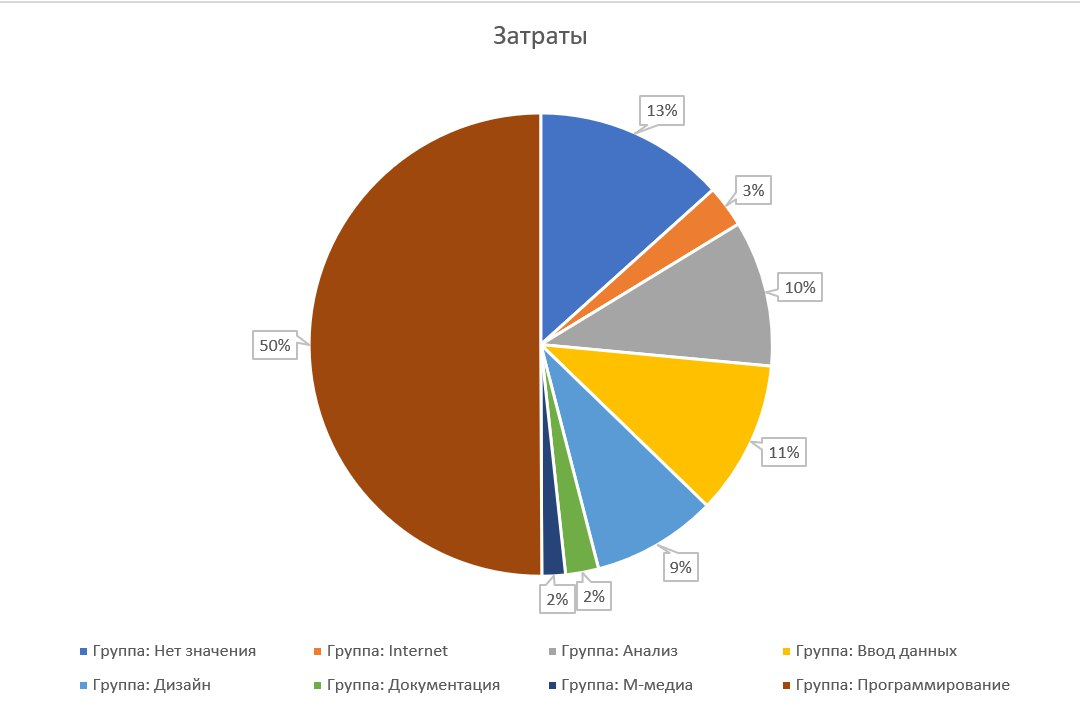
\includegraphics[scale=0.4]{inc/img/task3-costs-graph.jpg}
	\end{center}
	\captionsetup{justification=centering}
	\caption{Информации о затратах по структурным группам ресурсов из лабораторной работы № 2}
	\label{img:task3-costs-graph}
\end{figure}

Была проведена структуризация трудозатрат по группам ресурсов, как приведено на рисунке \ref{img:task3-new-labor-costs}. Графическое представление информации о трудозатратах по структурным группам ресурсов показано на рисунке \ref{img:task3-graph-labor}.

\begin{figure}[H]
	\begin{center}
		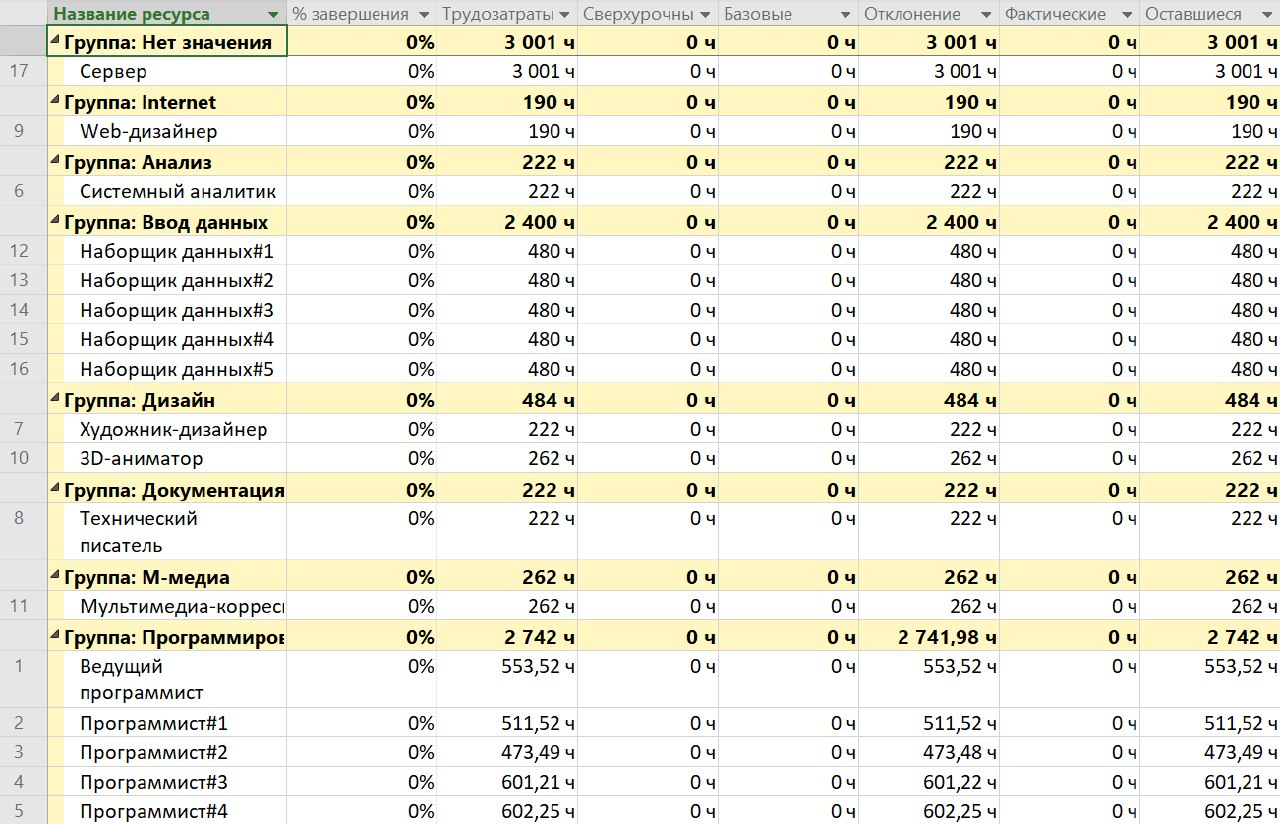
\includegraphics[scale=0.3]{inc/img/task3-new-labor-costs.jpg}
	\end{center}
	\captionsetup{justification=centering}
	\caption{Структуризация трудозатрат по группам ресурсов}
	\label{img:task3-new-labor-costs}
\end{figure}

\begin{figure}[H]
	\begin{center}
		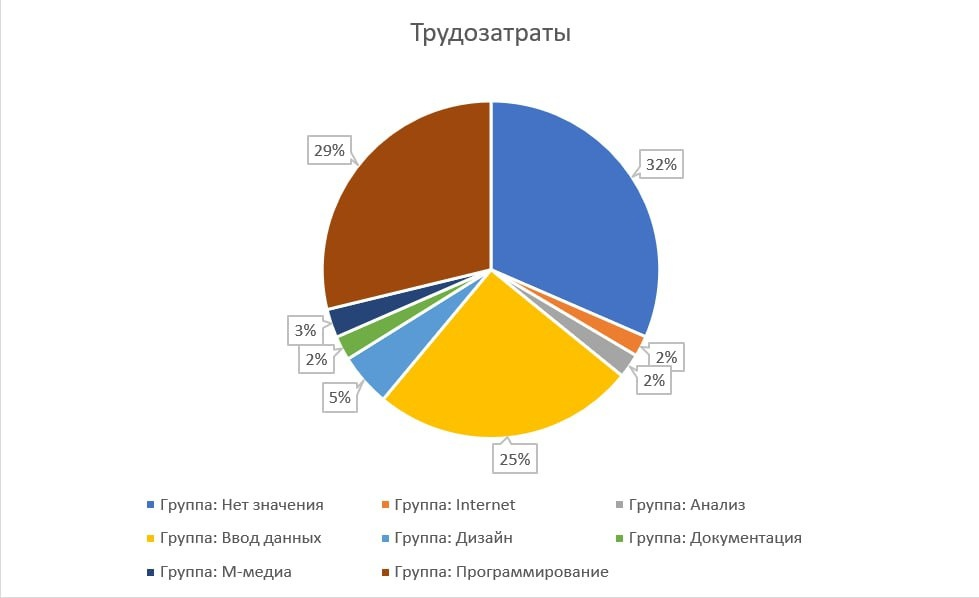
\includegraphics[scale=0.4]{inc/img/task3-graph-labor.jpg}
	\end{center}
	\captionsetup{justification=centering}
	\caption{Информации о трудозатратах по структурным группам ресурсов}
	\label{img:task3-graph-labor}
\end{figure}

\begin{figure}[H]
	\begin{center}
		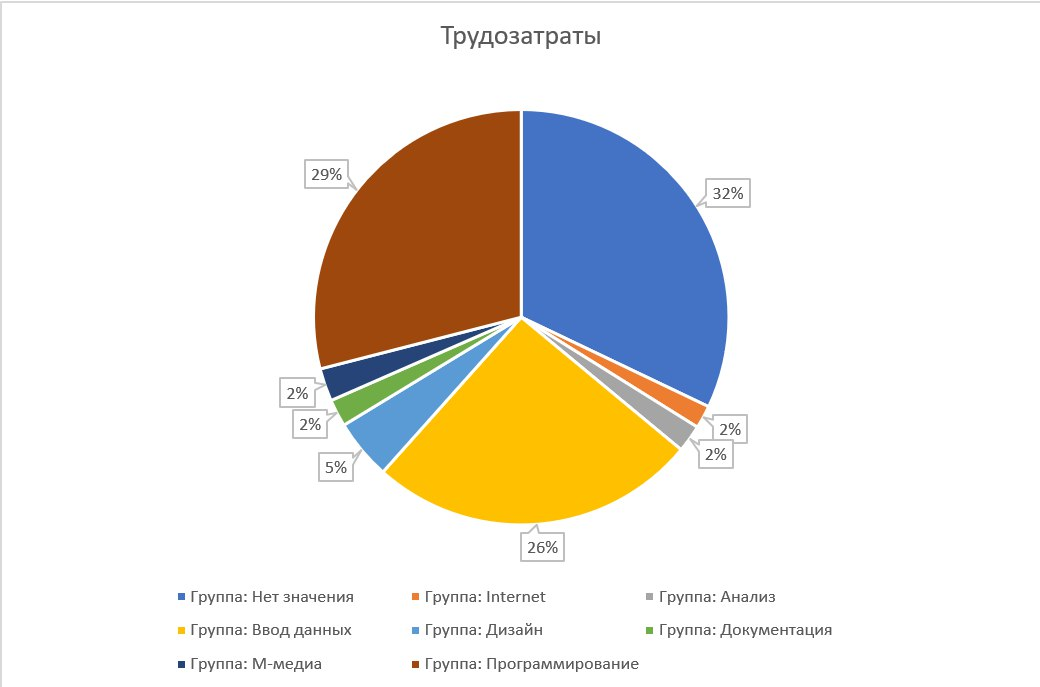
\includegraphics[scale=0.4]{inc/img/task3-labor-costs-graph.jpg}
	\end{center}
	\captionsetup{justification=centering}
	\caption{Информации о трудозатратах по структурным группам ресурсов из лабораторной работы № 2}
	\label{img:task3-labor-costs-graph}
\end{figure}

Изучив диаграммы, демонстрирующие распределение затрат и трудозатрат проекта, можно сделать следующие выводы:
\begin{itemize}
	\item удалось сократить на 2\% затраты группы <<Программирование>>;
	\item на 1\% увеличились затраты групп <<Анализ данных>> и <<Документация>>;
	\item удалось сократить на 1\% трудозатраты группы <<Ввод данных>>;
	\item на 1\% увеличились трудозатраты группы <<М-медиа>>.
\end{itemize}

Был сохранен базовый план проекта (рисунок \ref{img:task3-base}). При сохранении базового плана сохраняется полный набор предварительных оценок проекта, которые в дальнейшем будут использоваться для контроля за изменениями.

\begin{figure}[H]
	\begin{center}
		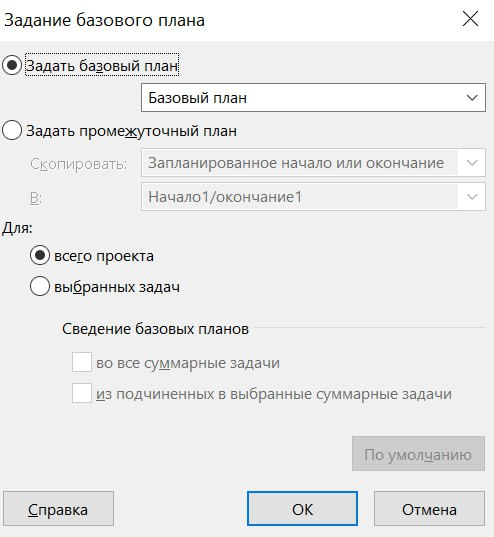
\includegraphics[scale=0.4]{inc/img/task3-base.jpg}
	\end{center}
	\captionsetup{justification=centering}
	\caption{Сохранение базового плана проекта}
	\label{img:task3-base}
\end{figure}

\section*{Вывод}

При выполнении лабораторной работы были отработаны навыки использования программы Microsoft Project для оптимизации временных и финансовых показателей проекта.

Проведя все оптимизации, удалось сократить бюджет проекта до 48 824.57 рублей и время проекта до 20.29 недель.
